\begin{frame}{Adaptation d'un maillage quad à une simulation}
    \begin{enumerate}
        \item Générer un premier maillage quad \( Q_0 \)
        \item Exécuter la simulation jusqu'à ce qu'elle échoue
        \item Calculer les champs de repère pour toutes les géométries intermédiaires de la simulation
        \item Calculer une paramétrisation
        \item Quantification et maillage quad
    \end{enumerate}
    
    % Ajouter une flèche en boucle
    \begin{tikzpicture}[overlay]
        \node (start) at (0.3, .65) {};  % Position de départ de la flèche
        \node (end) at (0.3, 2.9) {};    % Position d'arrivée de la flèche
        \draw[->, thick] (start) to[bend left=80] (end);
    \end{tikzpicture}
\end{frame}

\iffalse
\begin{frame}{Algorithm - Alternance maillage et simulation}
    \small
    \begin{algorithm}[H]
        \SetAlgoLined
        \label{algo:iterative_meshing_quadcover}
        \KwIn{Maillage de l'état initial de l'objet $Q_0$}
        \KwOut{Un maillage par pas de temps de la simulation $(Q_n)_{n \leq N}$}
        \SetKwProg{Fn}{Function}{:}{}
        \Fn{QuadcoverIteratif($Q_0$)}{
        $n_f \gets 0$\\
        \While{$n_f < N$}{
            Lancement de la simulation de déformation sur le maillage $Q_0$.\\
            $(Q_n)_{n \leq n_f} \gets$ un maillage quadrilatère par pas de temps réussi de la simulation\\
            \ForAll{$n \leq n_f$}{
                $T_n \gets Q_n$ divisé en un maillage triangulaire\\
            }
            $Q_0 \gets$ calcul d'un maillage initial adapté aux déformations $(T_n)_{n \leq N}$\\
        }
        \Return{$(Q_n)_{n \leq N}$}
        }
    \end{algorithm}
\end{frame}

\begin{frame}{Déterminer des valences de bord adaptés à la déformation}
    \small
    \begin{figure}
        \centering
        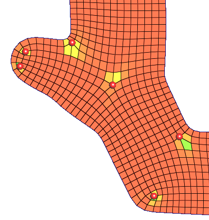
\includegraphics[width=0.46\linewidth]{img/quadsimu/coin_pb_0.PNG}
        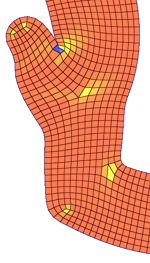
\includegraphics[width=0.27\linewidth]{img/quadsimu/coin_pb_1.PNG}
        \caption{Les positions de singularités optimales pour une géométrie initiale peuvent conduire à des quadrilatères de mauvaise qualité après une déformation.}
        \label{fig:asp_ratio_pb}
    \end{figure}
\end{frame}
\fi
\begin{frame}{Problème: Valences inadaptés à une déformation}
    \begin{figure}
        \centering
        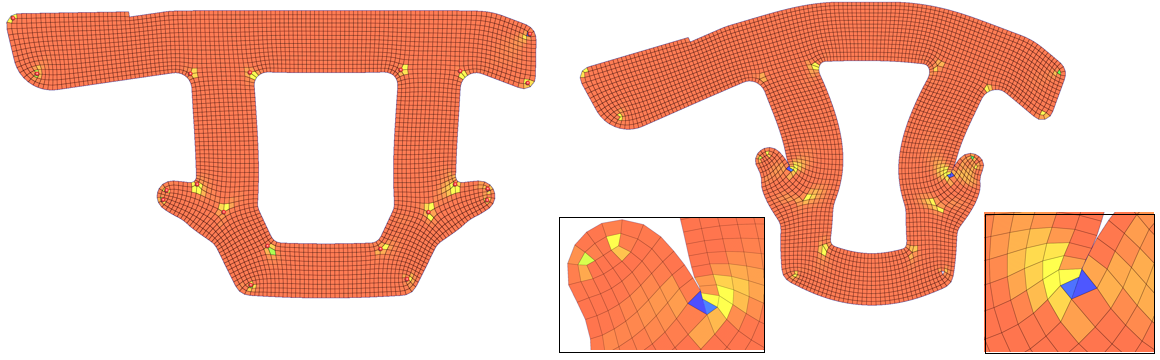
\includegraphics[width=\linewidth]{img/new_images/echec_simu.PNG}
        \caption{Les positions de singularités optimales pour une géométrie initiale peuvent conduire à des quadrilatères de mauvaise qualité après une déformation.}
    \end{figure}
\end{frame}
\begin{frame}{Déterminer des valences de bord adaptés à la déformation}
    \begin{columns}[c] % Le paramètre 'c' centre verticalement le contenu

        \column{0.5\textwidth}  % Largeur de la colonne de gauche
        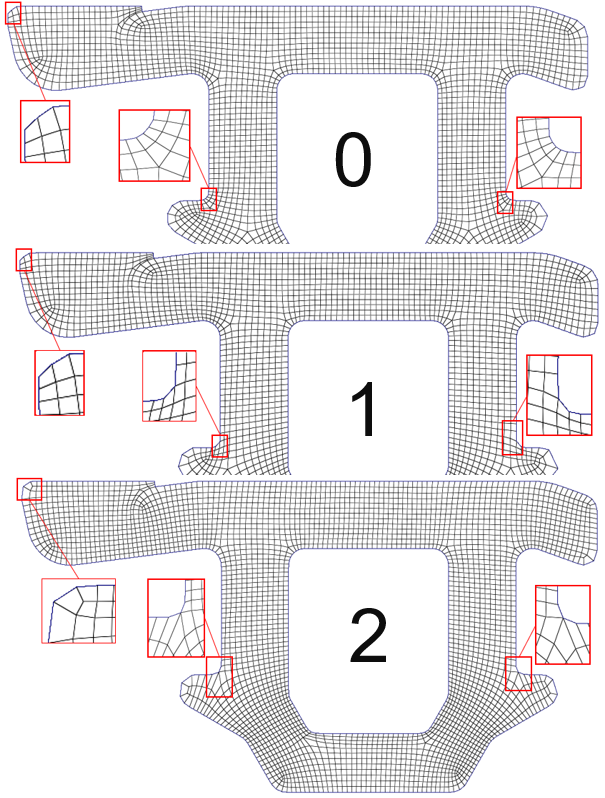
\includegraphics[width=\linewidth]{img/new_images/evolution_verrin.PNG}

        \column{0.5\textwidth}  % Largeur de la colonne de droite
        \only<1>{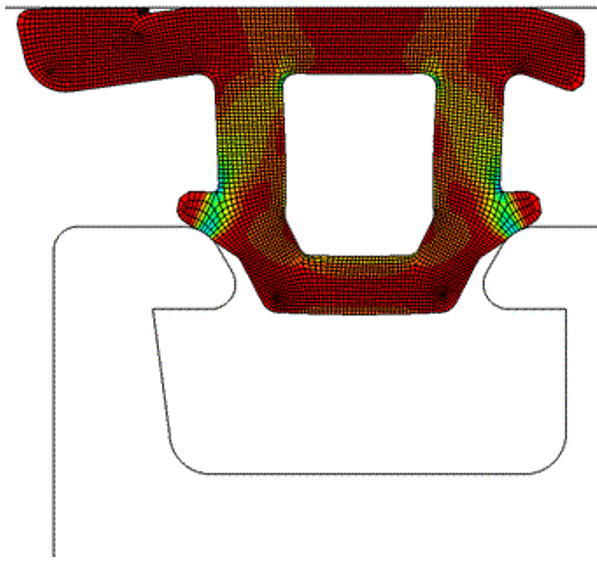
\includegraphics[width=\linewidth]{img/new_images/simu_debut_verrin.PNG}}
        \only<2>{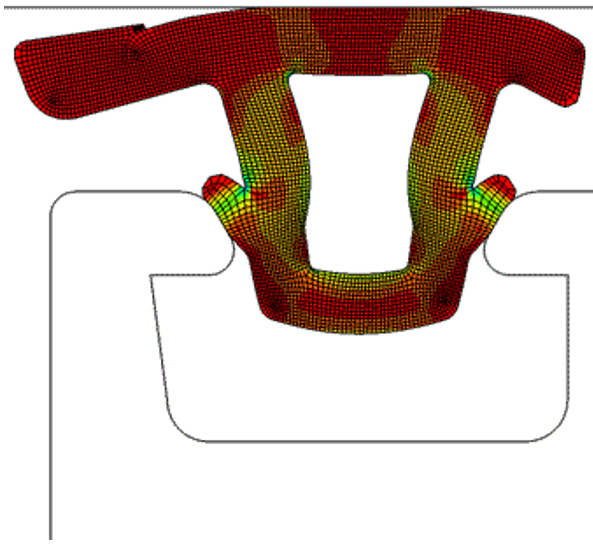
\includegraphics[width=\linewidth]{img/new_images/simu_milieu_verrin.PNG}}
        \only<3>{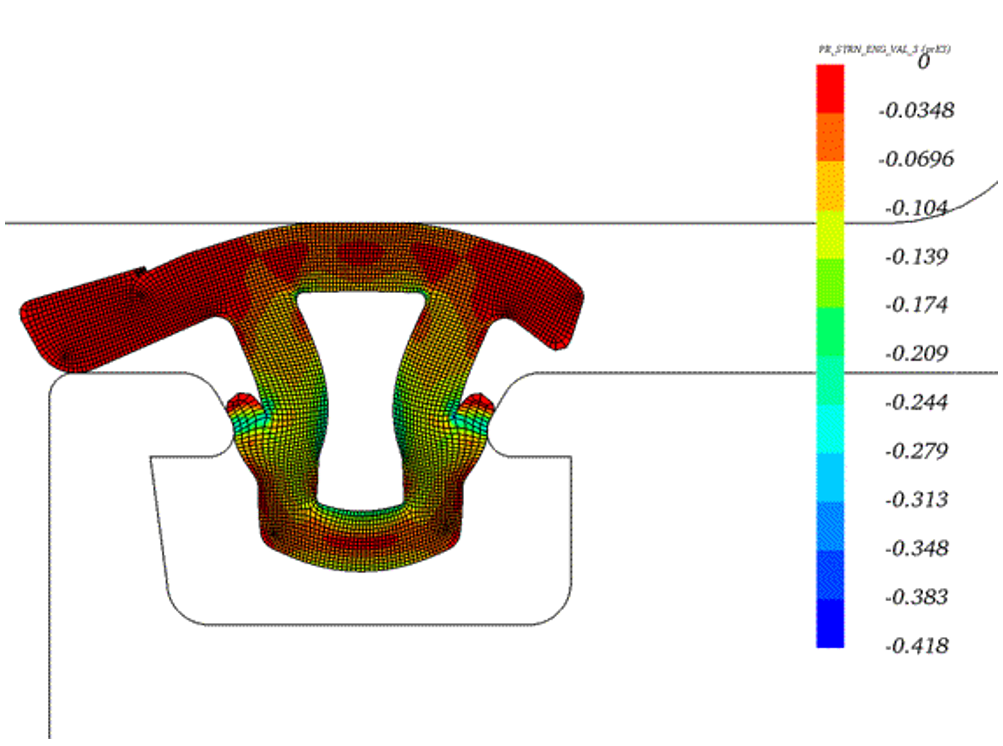
\includegraphics[width=\linewidth]{img/new_images/simu_fin_verrin.PNG}}
    \end{columns}
\end{frame}
\begin{frame}{Intégration à plusieurs géométries en entrée}
    \centering
    \only<1>{\textbf{Intégration de \blue{a} et \red{b} pour une géométrie}
    $$\argmin_{\blue{u}, \red{v}} \sum_{t, h} 
        \left\| \begin{pmatrix} \blue{u_{next(h)} - u_h} \\ \red{v_{next(h)} - v_h} \end{pmatrix}  - \begin{pmatrix} 
            < \blue{a_t}, \green{g_{next(h)} - g_h} > \\ < \red{b_t}, \green{g_{next(h)} - g_h} >\end{pmatrix} \right\|^2 $$}
    
    \only<2>{
        \textbf{Intégration de \blue{a} et \red{b} pour $N$ géométries}
    $$\argmin_{\blue{u}, \red{v}} \sum_{n\leq N} \sum_{t, h} 
        \left\| \begin{pmatrix} \blue{u_{next(h)} - u_h} \\ \red{v_{next(h)} - v_h} \end{pmatrix}  - \begin{pmatrix} 
            < \blue{a_{t, n}}, \green{g_{next(h), n} - g_{h, n}} > \\ < \red{b_{t, n}}, \green{g_{next(h), n} - g_{h, n}} >\end{pmatrix} \right\|^2 $$}

    \begin{columns}
        \begin{column}{0.5\textwidth}
            \begin{itemize}
            \item \( t \) : triangles du maillage
            \item \( h \) : demi-arêtes de \( t \)
            \item \( g \) : coordonnées (x, y)
            \end{itemize}
        \end{column}
    
        \begin{column}{0.5\textwidth}
            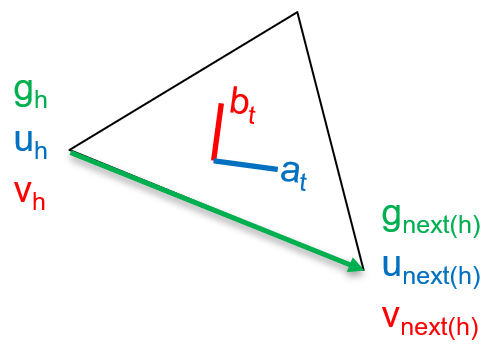
\includegraphics[width=.8\linewidth]{img/new_images/tri_g_u_v.PNG}
        \end{column}
    \end{columns}
\end{frame}
\iffalse
\begin{frame}{Carte sans couture adapté à la déformation}
    On fait la moyenne des $N$ champ de repère: 
    $$ \mu_i = \frac{1}{N} \sum_{n \leq N} \mu_{i, n} $$
    \pause
    On calcule une carte sans couture $u$ la plus proche possible de $\mu$:
    \begin{equation*} \label{eq:quadcover_energy}
        \begin{array}{ll}
            \underset{u}{\argmin} & \underset{t \in T}{\sum}\ \ \only<3>{\textcolor{red}{\lambda_t}} \underset{i, j \in \mathcal{C}(t)}{\sum} \left|\left| (u_i - u_j) - (\mu_i - \mu_j)  \right|\right|^2\\
            \text{sous contrainte: } & \begin{pmatrix} u_{i'} - u_{j'} \end{pmatrix} = R_{tt'} \begin{pmatrix}  u_{i} - u_{j} \end{pmatrix}. \\
        \end{array}
    \end{equation*}
    \pause
    Une carte sans couture est valide, si pour tout triangle $t$ et ses coins $i, j, k$:
    \begin{equation*}\label{eq:positive_jacobien_2D}
        \det \left(u_{j} - u_{i}, u_{k} - u_{i} \right) > 0
    \end{equation*}
\end{frame}
\fi

\begin{frame}{Résultats: Maillage quadrilatère avant et après adaptation}
    \begin{figure}
        \centering
        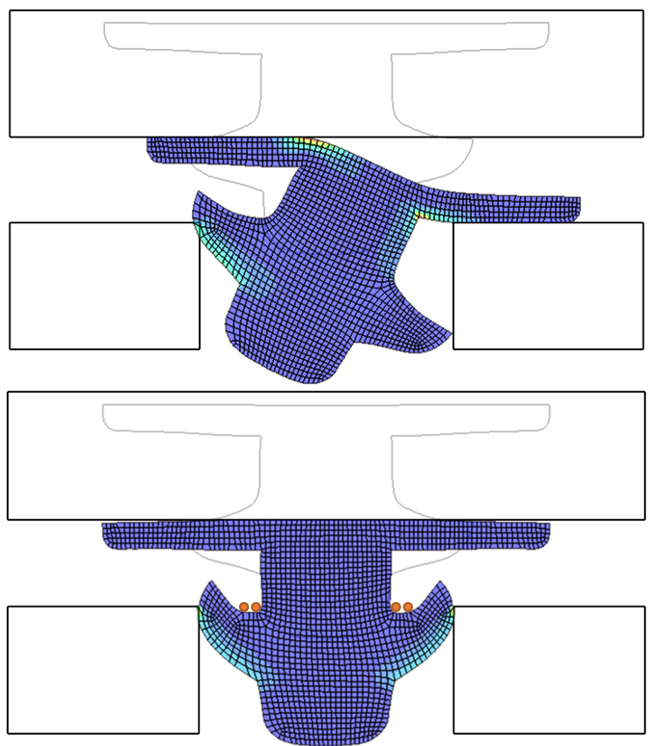
\includegraphics[width=0.5\linewidth]{img/quadsimu/deformation_same_step.PNG}
    \end{figure}
\end{frame}
 \iffalse
\begin{frame}{Adaptation progressive à la déformation}
    \begin{figure}
        \centering
        \only<1>{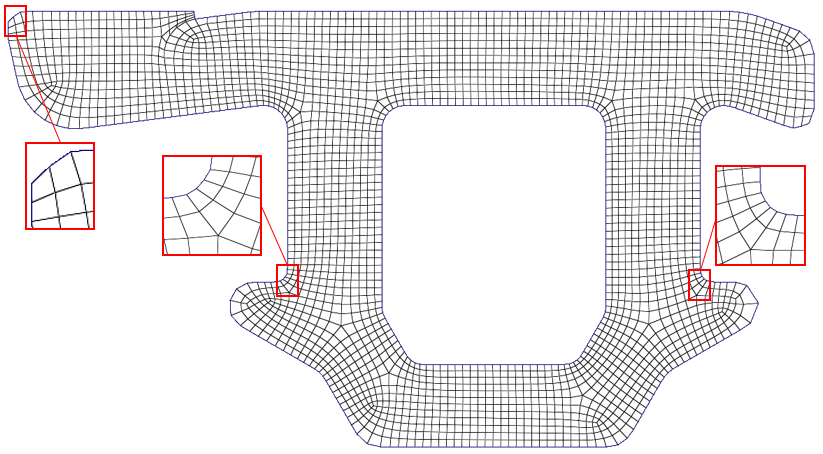
\includegraphics[width=0.69\linewidth]{img/quadsimu/seal_simu_1.PNG}}
        \only<2>{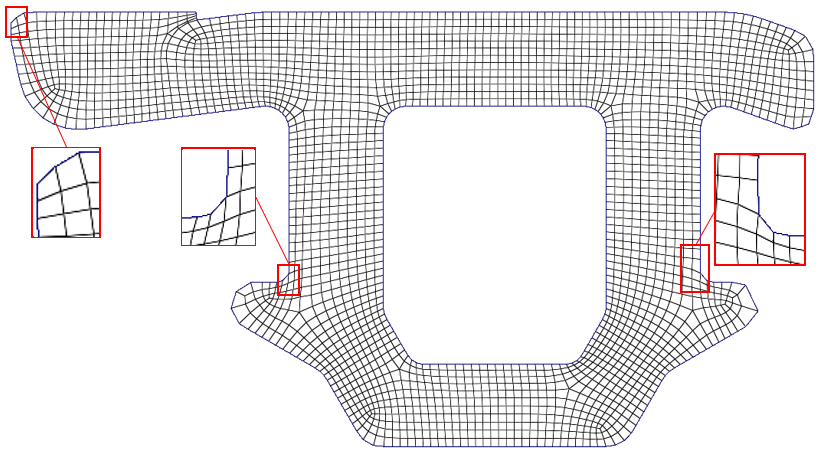
\includegraphics[width=0.69\linewidth]{img/quadsimu/seal_simu_2.PNG}}
        \only<3>{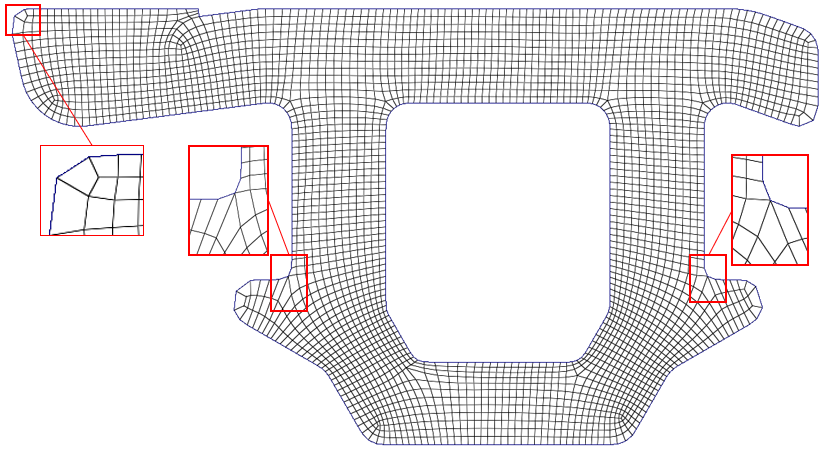
\includegraphics[width=0.69\linewidth]{img/quadsimu/seal_simu_3.PNG}}
    \end{figure}
\end{frame}
\fi

\begin{frame}{Résultats: comparaison avec une autre méthode automatique}
    \begin{figure}
        \centering
        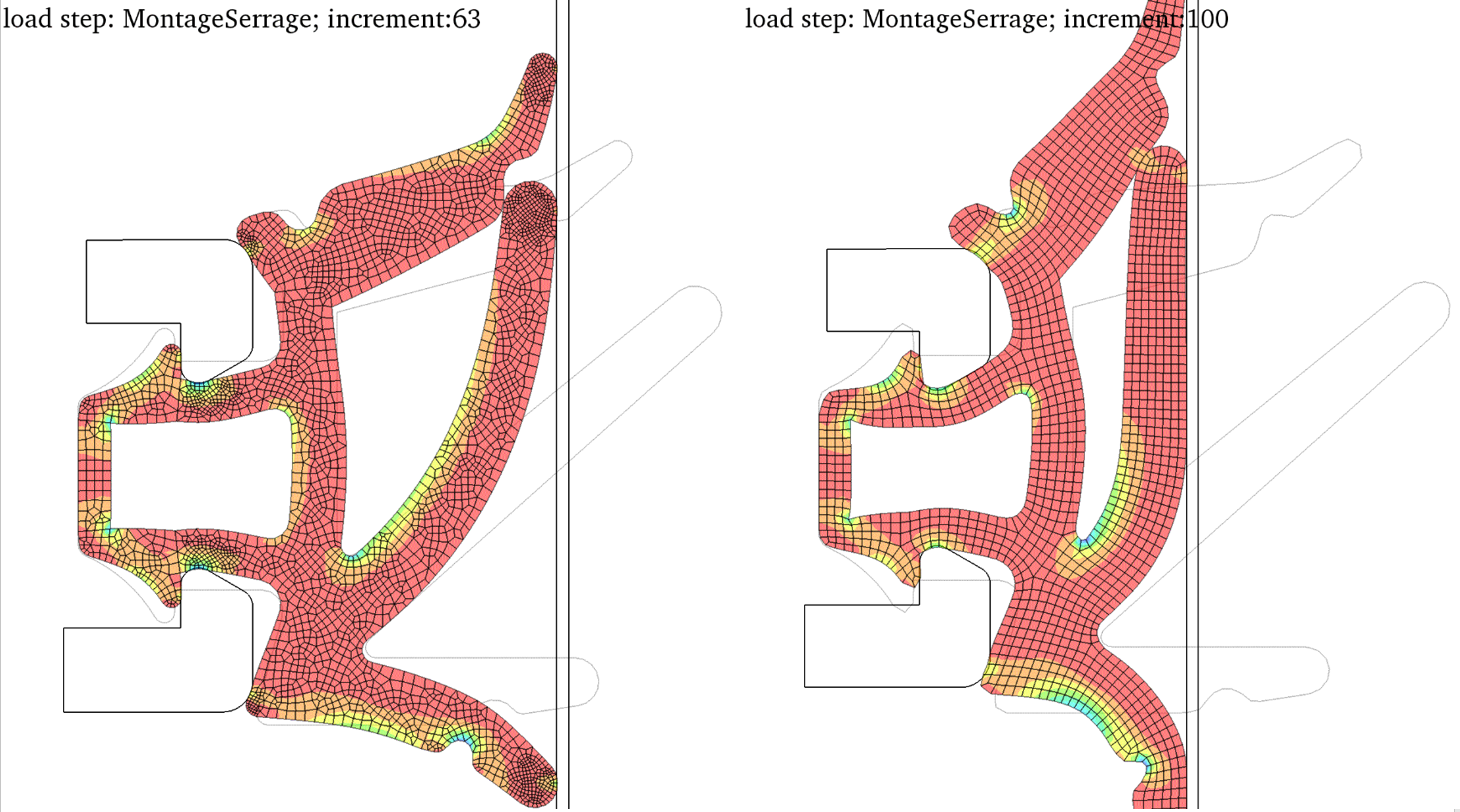
\includegraphics[width=0.99\textwidth]{img/quadsimu/comparison_with_bad_quality_mesh.PNG}
    \end{figure}
\end{frame}

\begin{frame}{Résultats: comparaison avec une méthode semi-manuelle}
    \begin{figure}
        \centering
        \only<1>{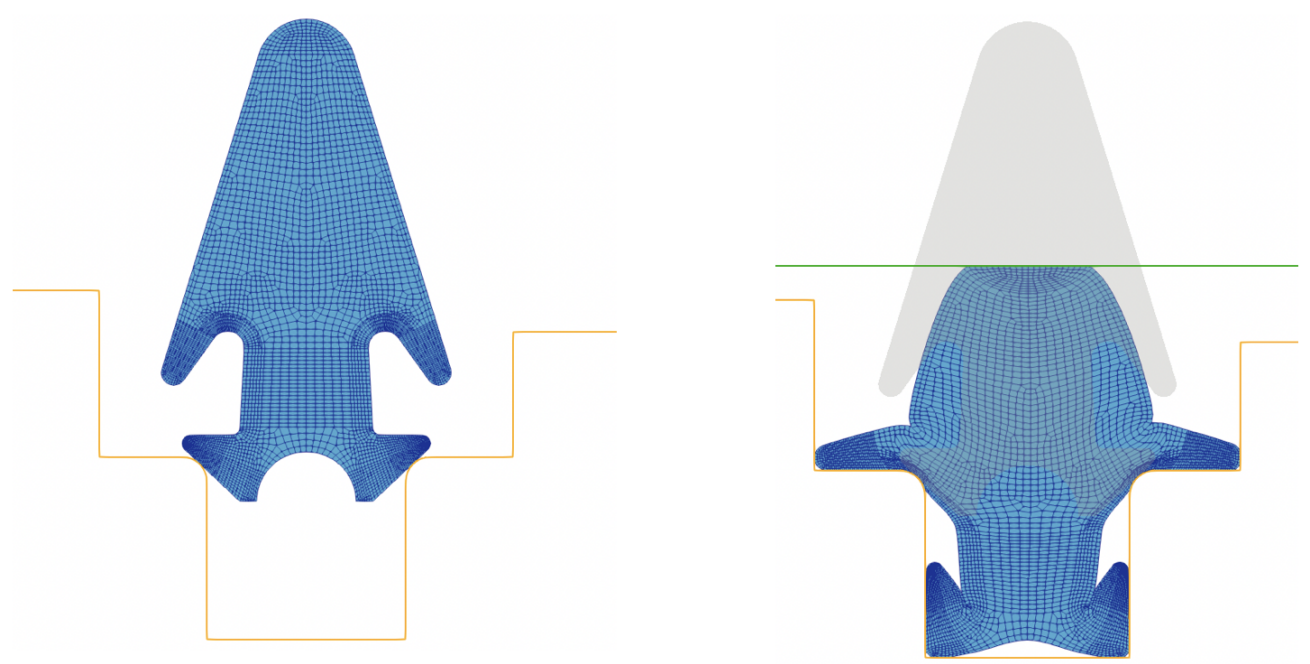
\includegraphics[width=0.99\textwidth]{img/introduction/hutchinson_sapin.PNG}}
        \only<2>{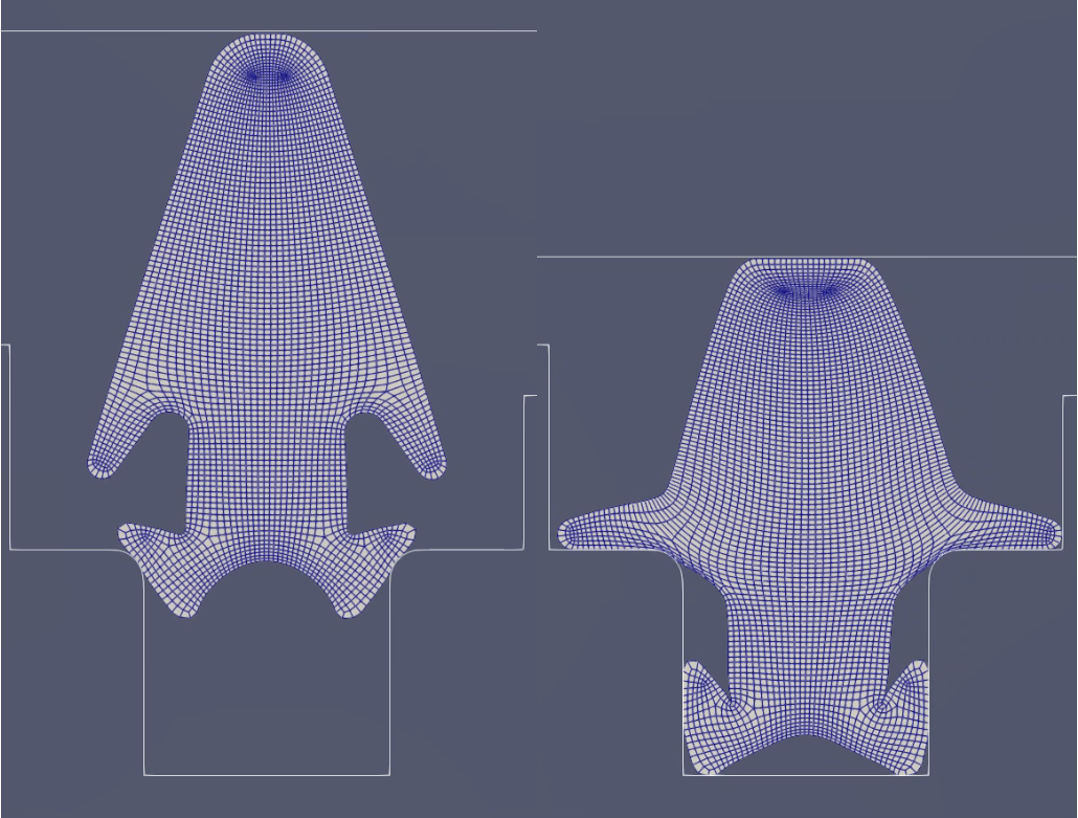
\includegraphics[width=0.79\linewidth]{img/quadsimu/resistance_to_compression.PNG}}
	\end{figure}
\end{frame}